\documentclass{article} % For LaTeX2e
% We will use NIPS submission format
\usepackage{nips13submit_e,times}
% for hyperlinks
\usepackage{hyperref}
\usepackage{url}
% For figures
\usepackage{graphicx} 
\usepackage{subfigure} 
% math packages
\usepackage{amsmath}
\usepackage{amsfonts}
\usepackage{amsopn}
\usepackage{ifthen}
\usepackage{natbib}

\title{Project-I by Group Sydney}

\author{
Diego Antognini \& Jason Racine\\
EPFL \\
\texttt{diego.antognini@epfl.ch}, \texttt{jason.racine@epfl.ch} \\
}

% The \author macro works with any number of authors. There are two commands
% used to separate the names and addresses of multiple authors: \And and \AND.
%
% Using \And between authors leaves it to \LaTeX{} to determine where to break
% the lines. Using \AND forces a linebreak at that point. So, if \LaTeX{}
% puts 3 of 4 authors names on the first line, and the last on the second
% line, try using \AND instead of \And before the third author name.

\nipsfinalcopy 

\begin{document}

\maketitle

\begin{abstract}
This report provides a summary of the project one of the PCML class. The project consists of doing regression and classification. For the regression data set we have observed that it was essential to separate the data into three clusters and doing a ridge regression on each of them due to the ill-condition matrix and the rapidity of tuning the algorithm. Moreover feature transformations like using polynomial basis was a key to decrease the prediction error. For the classification data set we have observed using logistic regression was as good as penalized logistic regression. Transformation of features in order to make them look like Gaussian as well as adding a polynomial basis help a lot to improve prediction accuracy.
\end{abstract}

\section{Regression}

\subsection{Data Description}

The train-data for regression consists of $N = 2800$ input ($\mathbf{X}$) and output ($\mathbf{y}$) data samples. Each input sample is a vector $\mathbf{x}_n$ with dimension $D = 76$. Out of these $76$ variables, $63$ are real, $3$ binary, $4$ categorical with 3 categories, $6$ are categorical with 4 categories.

We also have test-data of size $N=1200$ without their corresponding output. Our goal is to produce predictions for those data, as well as an approximation of the test-error.

\subsection{Data visualization and cleaning}

We first have plot the distribution of our features. As expected, they are not centered and we should normalize them. The Figure \ref{fig:histogram} shows an histogram of the output ($\mathbf{y}$) and we can conclude our data  seem to be a combination of three Gaussian distributions. It will be used later in order to separate the data in three sets and apply different regression models on them (each cluster will be normalized independently). We can also observe that each cluster have different sizes : 1946, 576 and 278. Moreover, on the right, we can see some data points (there are $2$) which have a higher values than the others. We consider them as outliers and will remove them.

\begin{figure}[!ht]
\vspace{-2em}
\center
\subfigure[Histogram of $\mathbf{y}$. We can see three Gaussian distributions and also some outliers on the right.]{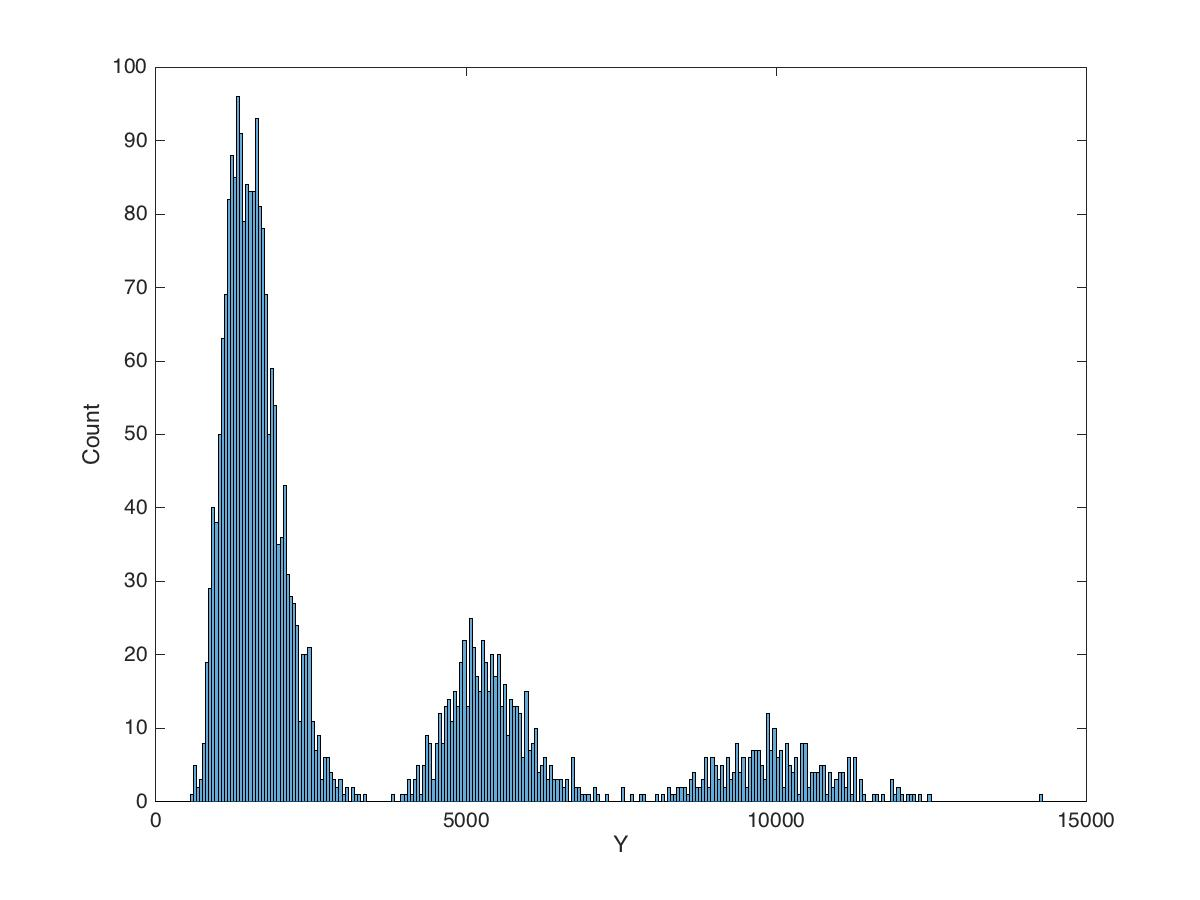
\includegraphics[width=2.7in]{figures/histogram.jpg} \label{fig:histogram}}
\hfill
\subfigure[Feature 2 can help us to separate the data. Green data points are misclassified data. The separation is at $x=0.42$.]{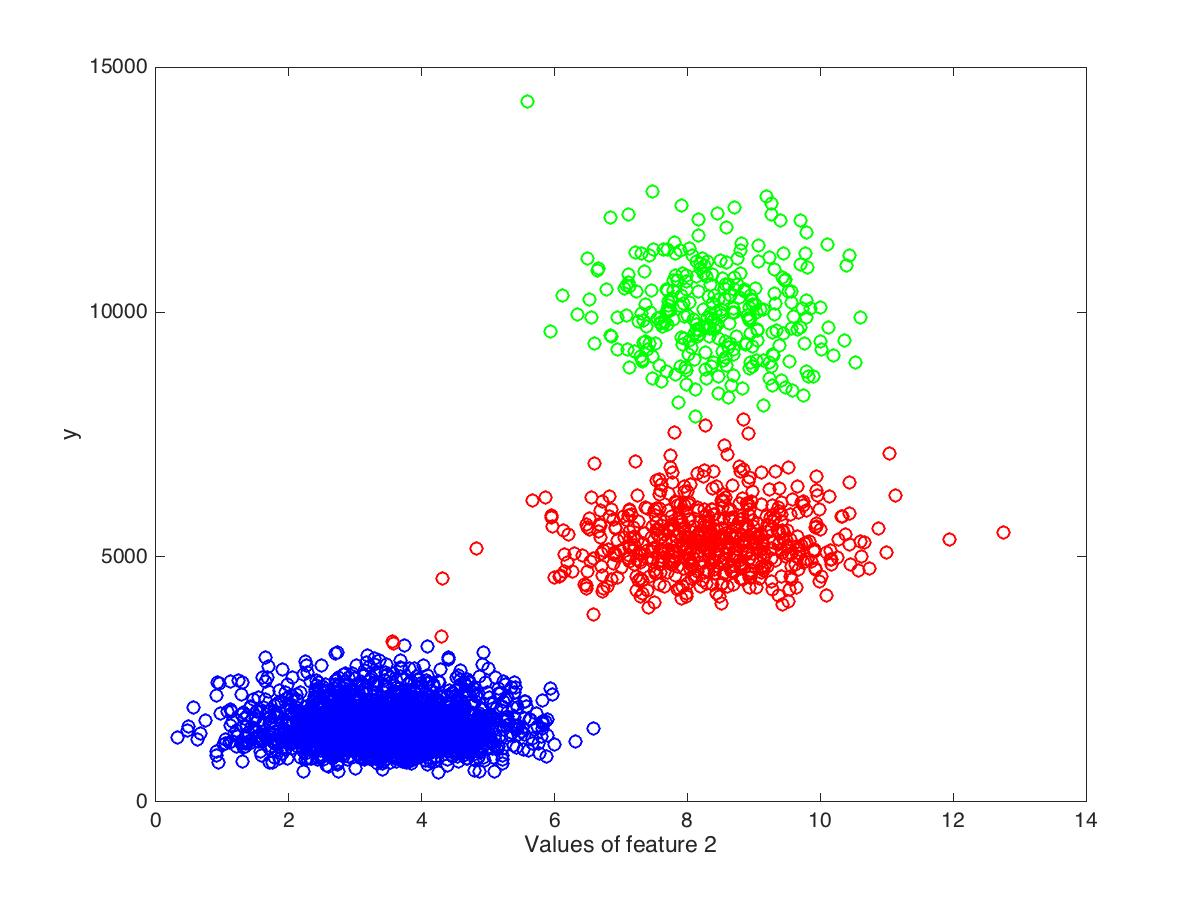
\includegraphics[width=2.7in]{figures/feature2.jpg}\label{fig:feature2}}
\hfill
\subfigure[Feature 16 can help us to separate the data. Green data points are misclassified data. The separation is at $x=1.17$.]{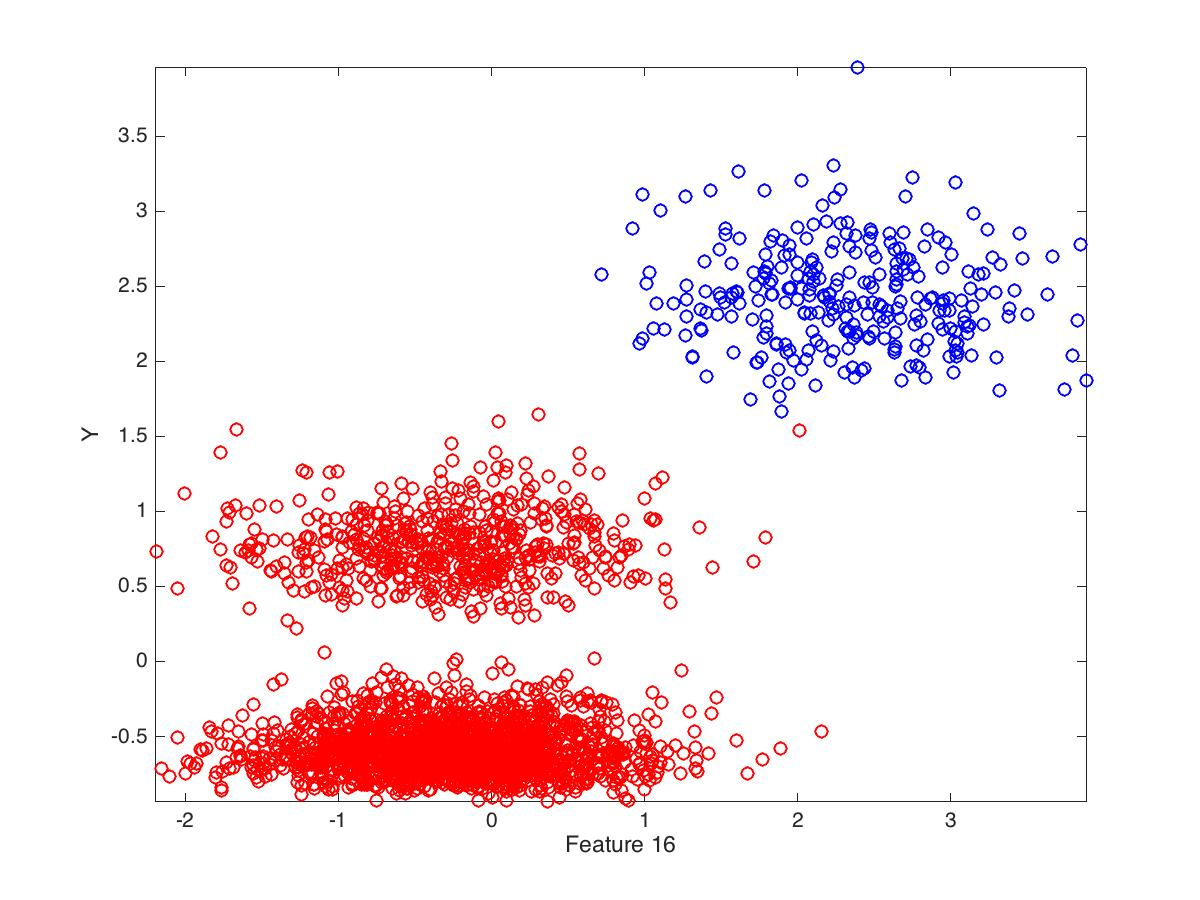
\includegraphics[width=2.7in]{figures/feature16.jpg}\label{fig:feature16}}
\hfill
\subfigure[Different degree for the polynomial basis of the cluster 1. We can observe a low variance. The third degree seems the best model to choose.]{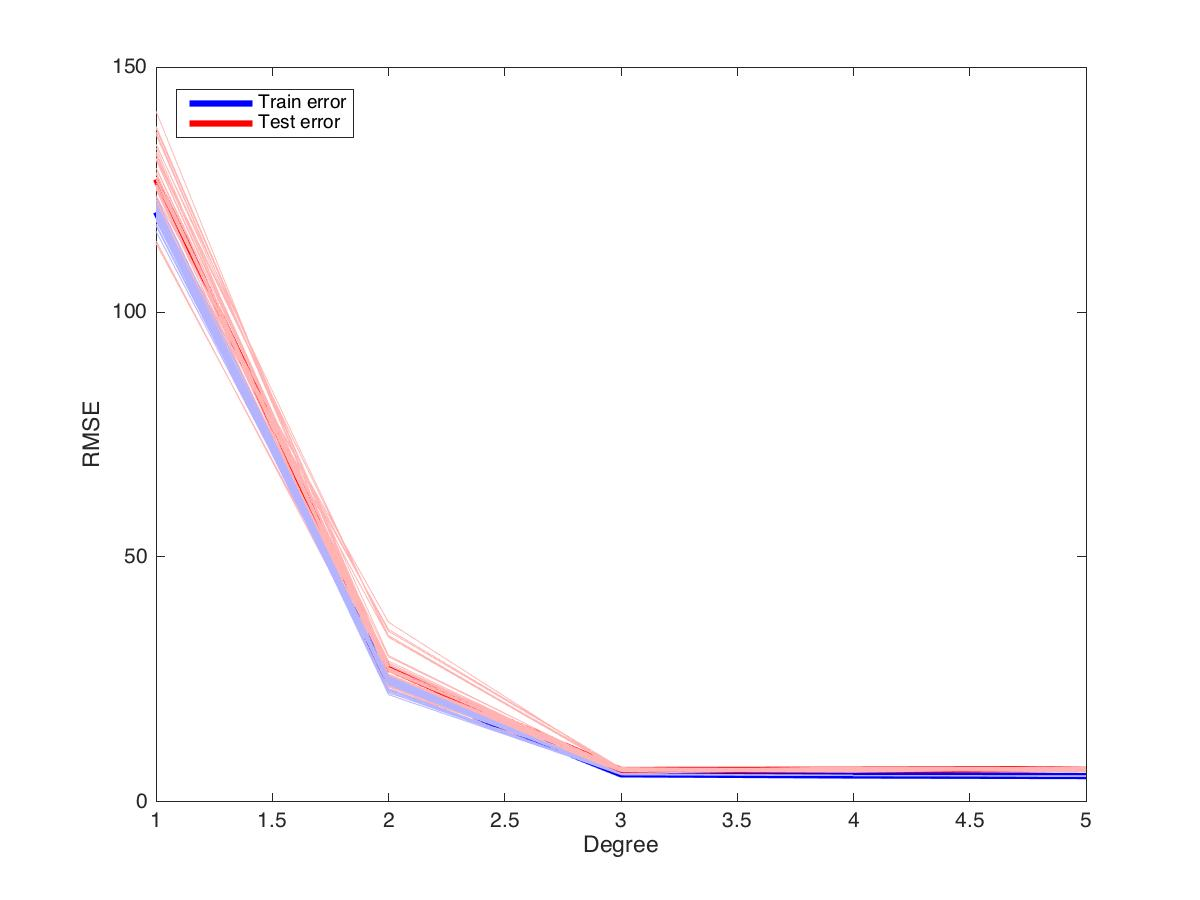
\includegraphics[width=2.7in]{figures/degrees_cls1.jpg}\label{fig:degrees_cls1}}
\vspace{-1em}
\caption{}
\end{figure}

To separate the data, we have observed that the feature $2$ and $16$ could help us. With Figure \ref{fig:feature2} we can see how we can use the second feature to separate cluster one to the others and observe $11$ misclassified data, which we will remove them in order to not corrupt our model. For the two other clusters, we need to observe the feature $16$. With Figure \ref{fig:feature16}, we can observe $14$ misclassified data. They also will be considered as outliers and removed. We set the threshold in order to minimize the number of misclassified data samples. Those thresholds are $0.42$ for the feature $2$ and $1.17$ for the feature $16$. So the final size of our clusters are $1937, 563$ and $273$.

We are also interested about the correlation between the input and output variables. We have observed the correlation for each cluster and conclude that for the first cluster, they are mainly in the range $[-0.1,0.1]$, except two features which are highly correlated. For the second and third cluster, also mainly in range $[-0.1,0.1]$ but this time, there are more correlated features (around 15). However, the features seem not have correlation between them.

We use dummy encoding for the categorical variables (for a categorical variable of size $k$, we need $k-1$ features), which gives us a total of $93$ input variables.

We can note that the rank of our input matrix $\mathbf{X}$ is rank-deficient with a rank of 66 instead of 76, and is rank-deficient of 65 for each cluster.
\vspace{-0.5em}
\subsection{Ridge Regression}

Since our matrix is ill-conditioned, using the least squares with normal equation wasn't suitable. Moreover, the results obtained were less good compared to the ridge regression method, and so we will not report those. The method using the least squares with gradient descent is appropriated as well as ridge regression method, which is suitable because we could lift the eigenvalues in order to avoid ill-conditioned matrix. It is also faster and a little bit more efficient than least squares using gradient descent and so, only results obtained with this latter will be reported.

\subsection{Evaluation methods}

In order to evaluate our different models, we have split our data ($\mathbf{X}$) in two sets of $80\%$ and $20\%$, for the training and the test sets. We choose this percentage in order to have still enough data for the training set and also enough to estimate correctly our models on the testing set. We learn only on the training set and then use the test set in order to estimate the error using the \textit{RMSE}. Moreover, we have also used $k$ fold cross validation (see next section for the values of $k$) to tune the parameters up like lambda or the different polynomial degrees. We repeated the experiment $30$ times with different seeds in order to split the data in a unique random way for each trial and so try to have an unbiased estimation error. Finally, we made vary the lambda from $10^{-5}$ to $10^{5}$ with $500$ values in-between.

\subsection{Model comparison}

The Figure \ref{fig:models} represents the \textit{RMSE} for each models. The first model used is the constant one, which will allow us to compare improvements with other models. It simply returns the mean of the outputs and doesn't depend on the inputs. Our second model does a ridge regression on the overall data using $10$ fold cross validation, because we have a lot of data, splitting them into $10$ fold seems reasonable. As expected, this is much better than previous model because we take into account the input features. Next model (third) is similar to the second one except that we add normalization on the real inputs (it doesn't make sense to also normalize categorical variables). Normalization is often a necessity depending on the algorithms used (e.g. gradient descent ones). It improves only slightly but because this is a good practice, we decided to keep it.

\begin{figure}
\vspace{-1em}
\center
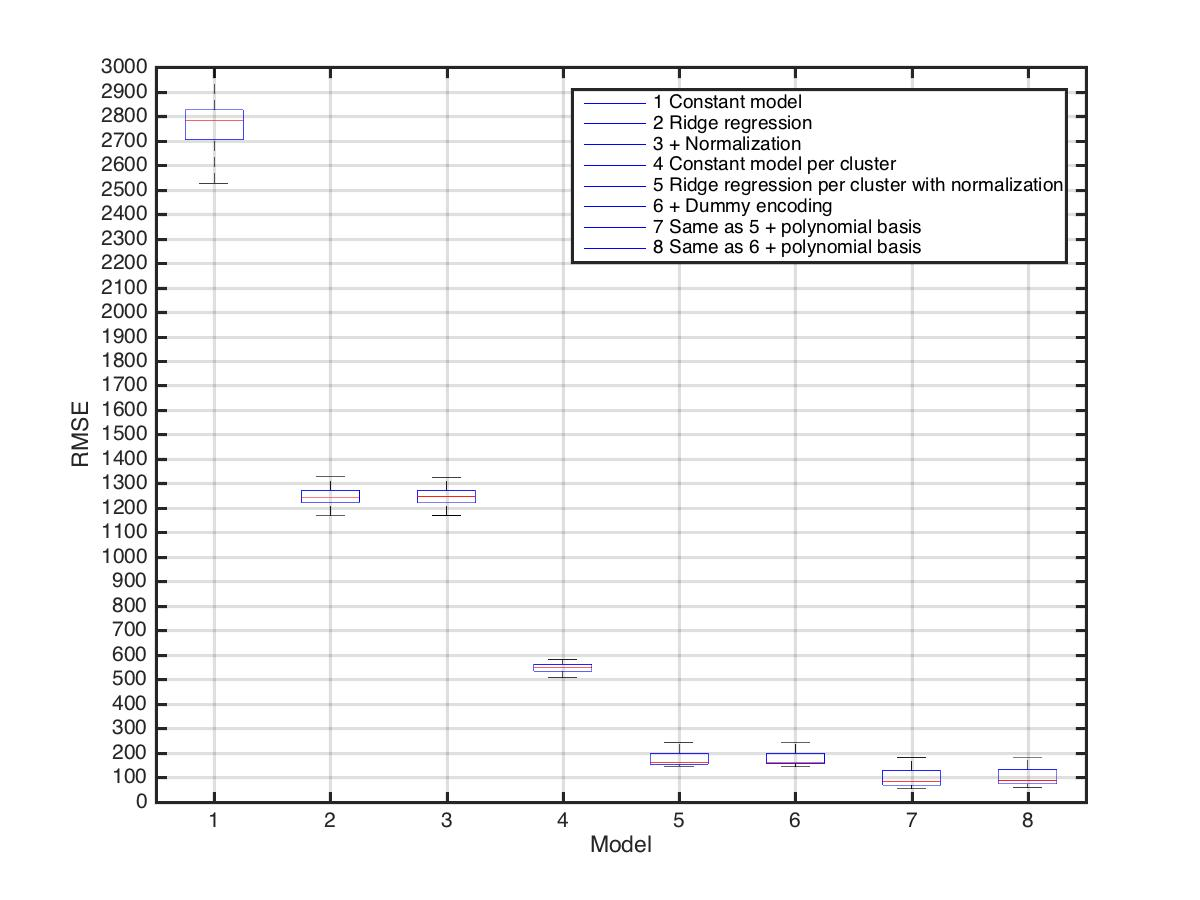
\includegraphics[width=4in]{figures/models.jpg} 
\vspace{-1em}
\caption{Boxplot of our models, using the RMSE. Each model is represented with a box where we can see their mean and their standard deviation.}
\label{fig:models}
\end{figure}

At this stage, we want to try to separate our data into clusters. The fourth model consists of using a constant model but this time separating the data into three clusters and then computing the mean for each cluster. We can observe a big improvement, justifying our choice to split the data into clusters. The next model (fifth) is about doing a ridge regression per cluster, each one having its own lambda. We also use $k$ fold cross validation where the first cluster has a $k_1=10$ because we have a lot of data ($1937$), the second $k_2=6$, because we don't have a lot of data ($563$) and the last $k_3=4$ because we really a small number of data ($273$) and so we have to choose a smaller k. As expected we obtained another big improvement justifying again the choice of splitting the data.

The sixth model consists of using dummy encoding for the categorical variables. Unfortunately, we didn't get major improvements. We think that the reason why dummy encoding doesn't help is because we don't have a high bias and so, having more features doesn't help.

The two next models is about using polynomial basis functions for each cluster. Categorical variables aren't concerned, they are just replicated for each degree, because it doesn't make any sense to build polynomial for them.  We have to be careful about the polynomial degrees to avoid the case where $D > N$. Moreover, if we don't observe significant improvement between degrees, we keep the lowest one. The Figure \ref{fig:degrees_cls1}, shows the case for the first cluster, we can also see that the variance is very low (same observation for the third one, however the second one has higher variance). The seventh model doesn't use dummy encoding and the eighth does.

For the seventh model, the degrees of the polynomial for the clusters are $3,6$ and $3$. When we add higher degrees, we can directly observe overfitting because suddenly the training error decreases to a value near zero and the test errors grows exponentially, so with this manner we know that our degrees are not to high. The eighth model is similar to the seventh one, except that this time it uses dummy encoding and has lower degrees : $3,5$ and $2$, due to the number of input variables. We can see that feature transformations significantly improve the test error compared to other models. However, dummy encoding doesn't seem to more efficient, and so our final model will be the seventh. Our final lambdas are $\lambda_1 = 0.0369, \lambda_2 = 1.8303e^{-4}$ and $\lambda_3 = 0.0053$.

\subsection{Feature transformations}

In hope to minimize the error, we tried different feature transformations. The first try was adding polynomial of them self as $X = [X X^2 X^3 ...]$ for which each cluster has its own degree. We made vary the different degrees and also the lambdas in order to keep the lambda which minimizes the test error. We also try feature transformations where the degree is a root, but unfortunately it was worst.

We also thought about removing some uncorrelated features, we tried to remove the most uncorrelated ones and then remove also the second one etc, but unfortunately we didn't get improvements. We think that the reason is that a feature may not be correlated directly with the output however a combination of uncorrelated features might be highly correlated. 

\subsection{Summary}

We analyzed a regression data set with different methods and concluded that least squares wasn't a good approach due to the ill-conditioning and the least squares gradient descent was to slow and was less efficient than ridge regression. Separation of the data into clusters was essential in order to decrease the test error. Unfortunately, dummy encoding didn't help. However using polynomial basis helped to decrease the bias. Finally, the variance of cluster 1 and 3 are very low, the one for cluster 2 is a bit higher. We think that we have bias because we use ridge regression but we don't think it is too high because we have seen that adding features helps and at a certain points it wasn't efficient. The best model we have is the seventh one, and we estimate the \textit{RMSE} of the prediction to be around $115.96$ with a standard deviation of $45.59$. Finally, we think that our model is improvable, however we couldn't try other things in order to improve the estimation error, due to a lack of time.

\section{Classification}

\subsection{Data Description}

The train-data for classification consists of $N = 1500$ input ($\mathbf{X}$) and output ($\mathbf{y}$) data samples. Each input sample is a vector $\mathbf{x}_n$ with dimension $D = 25$. Out of these $25$ variables, $20$ are real, $3$ categorical with 2 categories, $1$ is categorical with 4 categories and $1$ is categorical with 5 categories.

We also have test-data of size $N=1500$ without their corresponding output. Our goal is to produce predictions for those data, as well as an approximation of the test-error (using \textit{RMSE}, \textit{0-1 loss} and \textit{logarithmic loss}) using logistic regression and penalized logistic regression methods.

\subsection{Data visualization and cleaning}
\begin{figure}
\center
\subfigure[Histogram of different feature types. We can see that the first and second look like a Poisson distribution (the second has maybe be transformed with negative sign) and the third one a Gaussian distribution.]{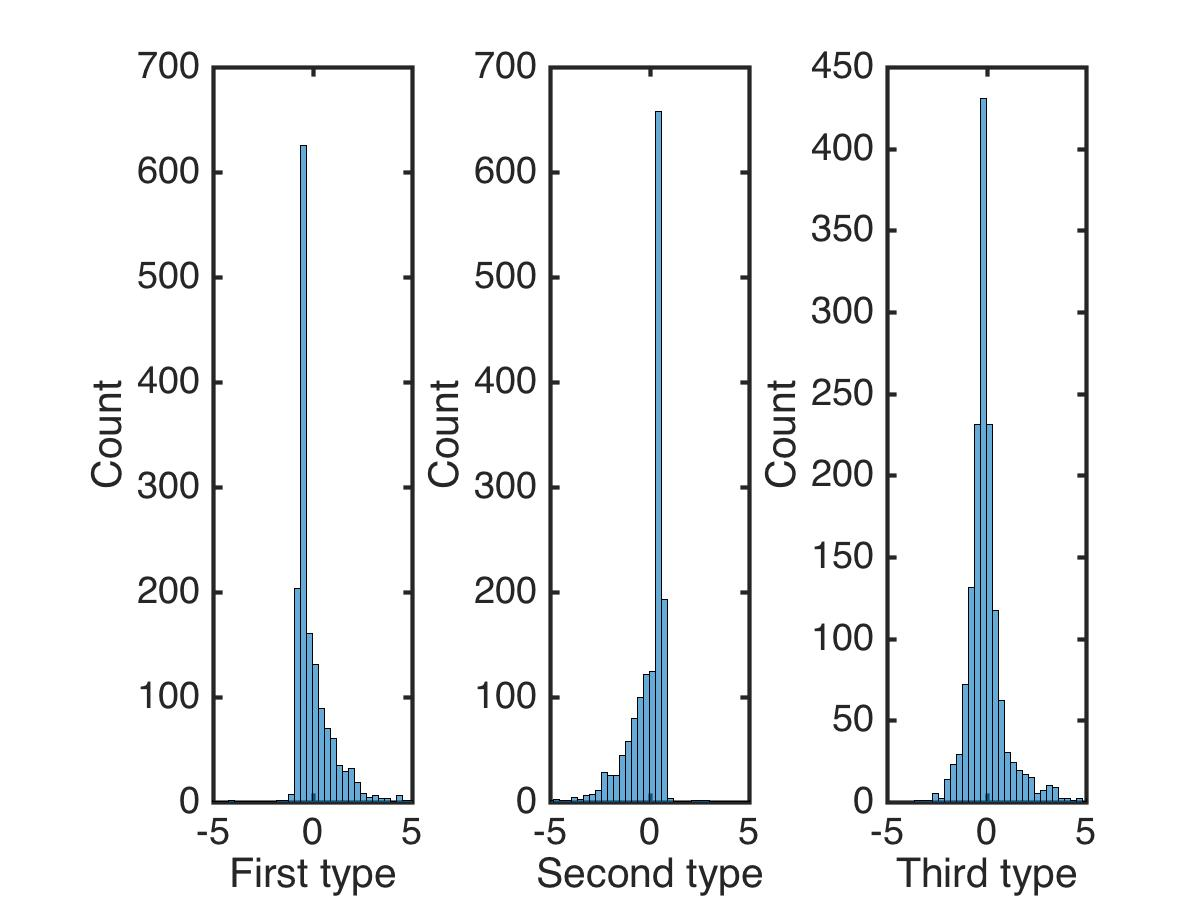
\includegraphics[width=2.65in]{figures/featuresType.jpg} \label{fig:featuresType}}
\hfill
\subfigure[Plot of the correlation of the features and the outputs. Some feature are highly correlated  whereas some have really low correlation.]{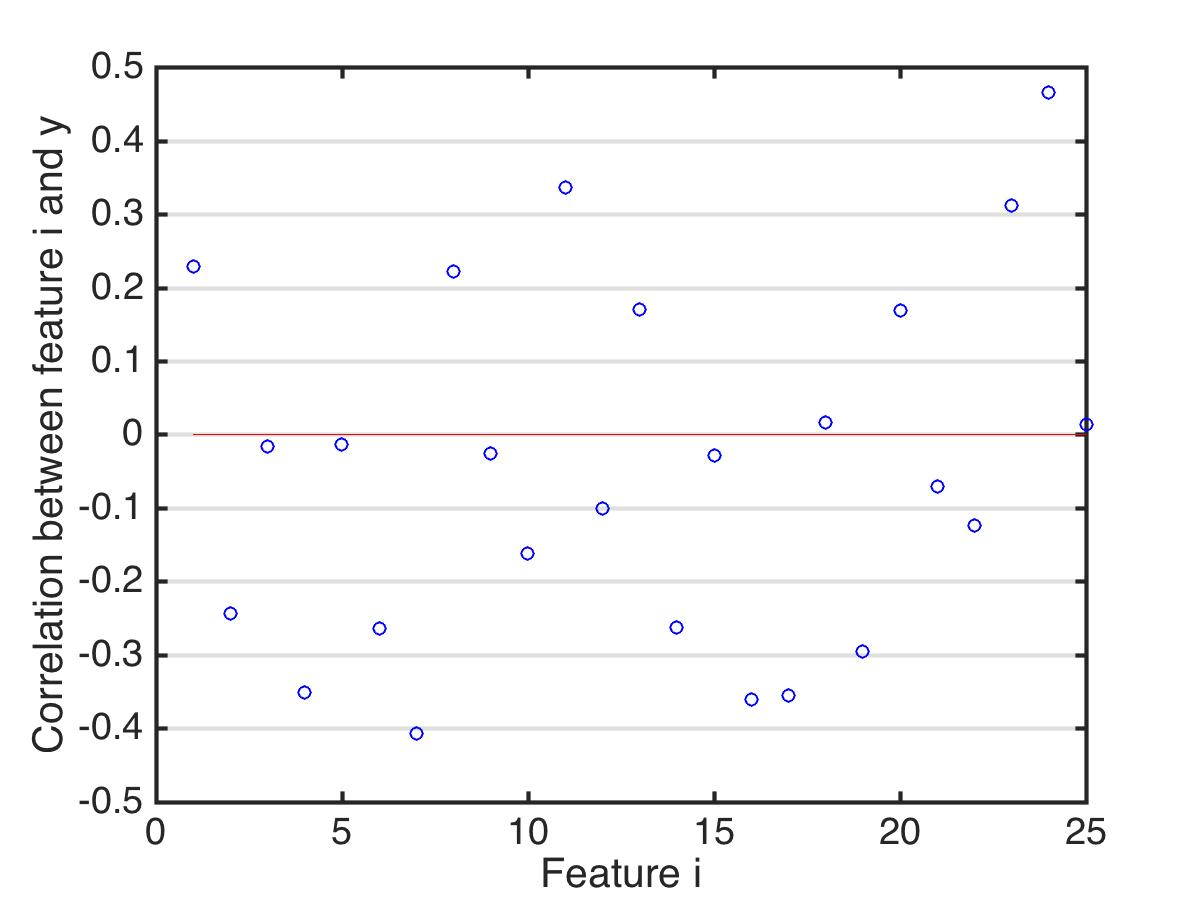
\includegraphics[width=2.65in]{figures/correlation.jpg} \label{fig:correlation}}
\caption{}
\end{figure}

We first have plot the distribution of our features. As expected, they are not centered and we should normalize them (good practice because we also use methods using gradient descents). Then we plot the histogram of the output which shows that approximately $64.8\%$ of the data are in a class and the other $35.2\%$ in another. We also plot the histogram of the categorical variables, which shows us that mostly their values are uniform. However, for the real features, we have distinguished 3 types : 1) Look likes a Poisson distribution where the peak is near 0 and the values are mainly positive 2) Same as one but the values are mainly negative and so, maybe they have been transformed with a negative sign from a Poisson distribution. 3) Look likes Gaussian distribution which is not centered. The Figure \ref{fig:featuresType} shows their histogram with their values normalized.

We use dummy encoding for categorical variables which gives us a total of $31$ input variables.

We are also interested about the correlation between the input and output variables. The Figure \ref{fig:correlation} shows the correlation. We have observed that the features are correlated mainly in the range $[-0.3,0.3]$ and some have higher correlation near $\pm0.4$ and $0.5$ like feature $7$ or $24$.We have decided to not remove features with low correlation because we don't have any pertinent reason to do so.

Finally, our matrix ($\mathbf{X}$) is a full-rank matrix, which is a good news for logistic regression.

\subsection{Logistic Regression}

Since our matrix is full-rank using logistic regression was appropriate. Because logistic regression is more efficient in term of complexity and that we don't need to penalize some betas, we report only the results using this method. However, using penalized logistic regression gave us similar results.

\subsection{Evaluation methods}

In order to evaluate our different models, the method is similar that the one used in regression. We split our data ($\mathbf{X}$) in two sets of $80\%$ and $20\%$, we compute the test-error using the \textit{RMSE}, \textit{0-1 loss} and \textit{logarithmic loss}. Because all the errors grows similarly and we think that \textit{0-1 loss} is the easiest error to visualize, we have decided to report only this error. To find the learning step $\alpha$, we have used $10$ fold cross validation because we have enough data to use this $k$. We repeated the experiment $30$ times with different seeds in order to split the data in a unique random way for each trial.

\subsection{Model comparison}

The Figure \ref{fig:models_classification} represents the \textit{0-1 loss} for each models. The first model used is the constant one, which will allow us to compare improvements with other models. It simply returns $1$ and doesn't depend on the inputs. Our second model does a logistic regression, using normalization, using only real features and transforming the output in the range $[0,1]$ because the logistic regression results are in this range. We can see that it clearly outperforms the constant model. In the next model (third) we added the categorical variables which didn't improve the error and increase a little bit the variance. However, because it could be important features, we have decided to keep them.

\begin{figure}
\center
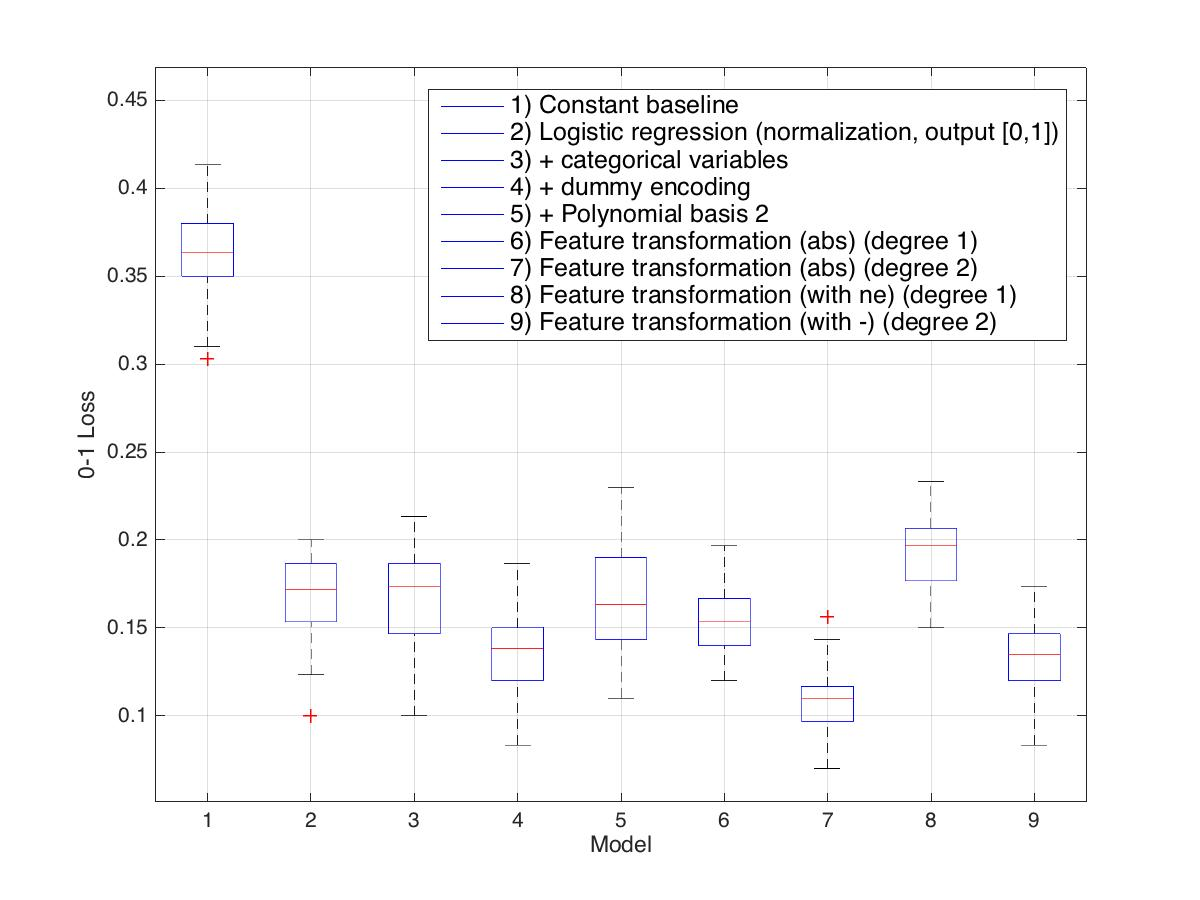
\includegraphics[width=4in]{figures/models_classification.jpg} 
\vspace{-1em}
\caption{Boxplot of our models, using the 0-1 Loss. Each model is represented with a box where we can see their mean and their standard deviation.}
\label{fig:models_classification}
\vspace{-0.5em}
\end{figure}

The fourth model consists in using dummy encoding for the categorical variable. This times, the error was improved and the variance has diminished. The next model (fifth) adds a polynomial basis of degree 2. We can observe the the variance as increased, we have some outliers (five in total, there might be hidden due to the legend) and the error has increased. We think that the bias is better but due to its high variance, we consider it as a bad model.

In order to try to improve the error, we have transformed the feature (more information in the next section) with the formula $\sqrt[4]{|x|}$ in order to have more Gaussian-like distribution. The sixth model represents this transformation. We can observe that the error is a little bit higher than model 4 but the mean is more stable and the variance lower. Because we assume that data samples are generated from a Gaussian distribution, we decided to continue this way. The seventh one adds a polynomial basis of degree 2, which improves the error and still decreases the variance. Moreover, because we use more features, we think that our model has also a lower bias.

The two last models (eighth and ninth) use another transformation where negative values weren't transformed into positive one, holding them with the formula $-\sqrt[4]{-x}$ and try using also a polynomial basis. However, the error wasn't as good as the seventh model, surely because the transformed feature look like less Gaussian than the transformation using the absolute values. We can also see that the variance seems also higher.
Our final model will be the seventh.

\subsection{Feature transformations}

In hope to minimize the error, we tried different feature transformations. The first try was add polynomial of them self as $X = [X X^2]$. With the data not transformed into Gaussian like distribution, we didn't get an improvement (even with degree 3). We then try to transform the features which look like a Poisson distribution in order to transform them into a Gaussian-like distribution. We first use the formula $\sqrt[4]{|x|}$ which gave us good results even if we transformed the negative values into positive. Mixed with polynomial of features at degree 2 allowed us to have an important improvement for the error. We also try to keep the negative values, using the formula $-\sqrt[4]{-x}$ but unfortunately, it didn't help. We think the reason is first that distribution was more a superposition of two Gaussian. Using a degree greater than 2 didn't improve the error, surely because our bias is not too high.

\subsection{Summary}

We analyzed a classification data set with different methods and concluded that logistic regression was appropriate because the input matrix was full-rank. Moreover, using the penalized logistic regression gave us similar results. Using normalization was essential as well as transforming the output in the range $[0,1]$. Adding categorical variables with dummy encoding helps. The key of our model was to transform features which look like Poisson distribution into a Gaussian like distribution using $\sqrt[4]{|x|}$ and using a polynomial basis of degree 2. We think that our model is improvable due to outliers because we couldn't find such outliers in all dimensions (or most of the dimensions). We estimate the mean and standard deviation of the prediction, using the \textit{RMSE},\textit{0-1 loss} and \textit{logarithmic loss} respectively to be around $0.329$, $0.109$ and $0.509$ for the mean, and $0.028$, $0.018$, $0.018$for the standard deviation .

\end{document}